\documentclass{article}



\usepackage{arxiv}

\usepackage[utf8]{inputenc} % allow utf-8 input
\usepackage[T1]{fontenc}    % use 8-bit T1 fonts
\usepackage{hyperref}       % hyperlinks
\usepackage{url}            % simple URL typesetting
\usepackage{booktabs}       % professional-quality tables
\usepackage{amsfonts}       % blackboard math symbols
\usepackage{nicefrac}       % compact symbols for 1/2, etc.
\usepackage{microtype}      % microtypography
\usepackage{lipsum}		% Can be removed after putting your text content
\usepackage{graphicx}
\graphicspath{ {./images/} }
\usepackage[square,numbers]{natbib}
\usepackage{doi}

\title{ZPY: Open Source Synthetic Data for Computer Vision}

\author{
	{\hspace{1mm}Hugo Ponte}\thanks{correspondence author} \\ 
	Zumo Labs \\
	\texttt{hugo@zumolabs.ai} \\
	\And
	{\hspace{1mm}Norman Ponte} \\
	Zumo Labs \\
	\texttt{norman@zumolabs.ai} \\
	\And
	{\hspace{1mm}Sammie Crowder} \\
	Zumo Labs \\
	\texttt{sammie@zumolabs.ai} \\
	\And
	{\hspace{1mm}Kory Stiger} \\
	Zumo Labs \\
	\texttt{kory@zumolabs.ai} \\
	\And
	{\hspace{1mm}Steven Pecht} \\
	Zumo Labs \\
	\texttt{steven@zumolabs.ai} \\
	\And
	{\hspace{1mm}Elena Ponte} \\
	Zumo Labs \\
	\texttt{elena@zumolabs.ai} \\
}

% Uncomment to remove the date
\date{}

\renewcommand{\headeright}{Technical Report}
\renewcommand{\undertitle}{Technical Report}

% PDF metadata
\hypersetup{
pdftitle={ZPY: Open Source Synthetic Data for Computer Vision},
pdfsubject={cs.CV},
pdfauthor={Hugo Ponte, Norman Ponte, Sammie Crowder, Kory Stiger, Steven Pecht, Elena Ponte},
pdfkeywords={Computer Vision, Synthetic Data, Machine Learning, Open Source, Python, Blender},
}

\begin{document}
\maketitle

\begin{abstract}
Synthetic data presents a unique solution to the huge data requirements of computer vision with deep learning.
In this work, we present zpy \citep{zpy}, an open source framework for creating synthetic data. Built on top of Blender,
and designed with modularity and readability in mind.
\end{abstract}

\keywords{Computer Vision \and Synthetic Data \and Machine Learning \and Open Source \and Python \and Blender}

% https://www.overleaf.com/learn/latex/Inserting_Images
\begin{figure}[!ht]
	\centering
	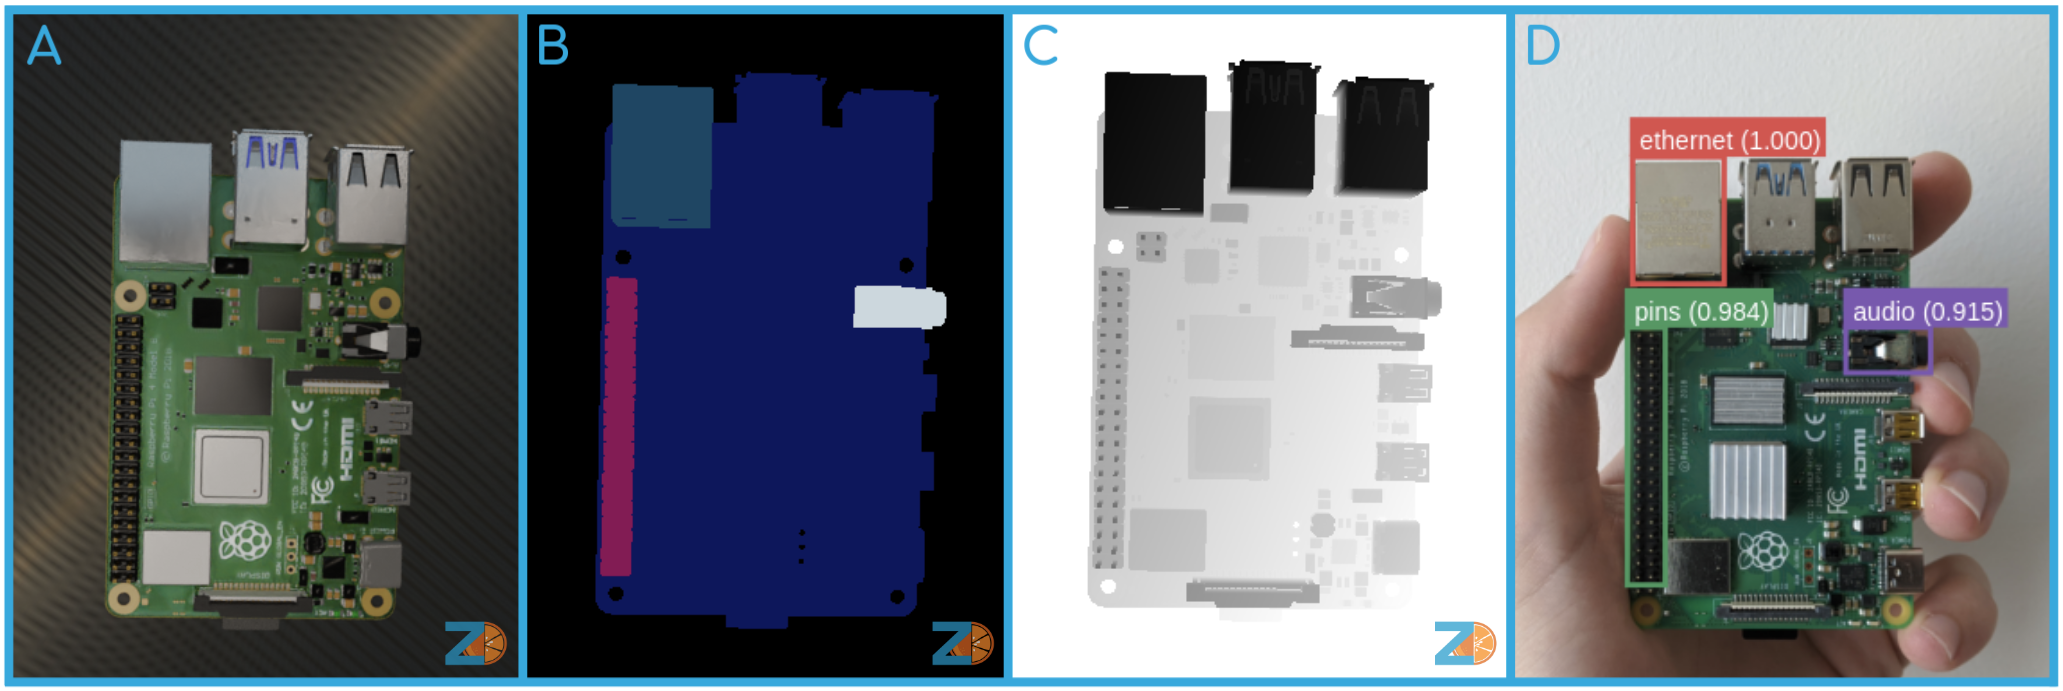
\includegraphics[width=\textwidth]{cover.png}
	\caption{Synthetic images of a raspberri pi created with zpy: (A) color image, (B) segmentation image, (C) depth image, (D) prediction image}
	\label{fig:fig1}
\end{figure}

\section{Introduction}
\label{sec:introduction}
\lipsum[2]

\section{Background}
\label{sec:background}
\lipsum[2]

\subsection{3D}

3D, short for the three dimensions of space we experience,  is a catch-all term used to describe the
 varied technologies used to create virtual worlds. The earliest uses of 3D were in the engineering 
 world for design and manufacturing. A huge use case for 3D has emerged in entertainment, where 
 virtual worlds are created for movies and games. More recently, the 3D stack has been used to power 
 emerging technologies such as robotics, VR/AR, and deep learning.

\subsubsection{Asset Creation}
\lipsum[5]

\subsubsection{Asset Scripting}
\lipsum[5]

\subsection{Deep Learning}
Modern deep learning can be implemented in a variety of programming languages including Python, R, Julia,
 Scala, Ruby, Octave, MATLAB, and even C/C++. Amongst these, Python has emerged as the lingua franca,
  rising to the top in part due to the popularity of open source frameworks such as
  TensorFlow \citep{tensorflow}, PyTorch \citep{pytorch}, and Scikit-Learn \citep{scikit-learn}.

\subsection{Synthetic Data}
\lipsum[5]

\section{Motivation}
\label{sec:motivation}

\subsection{Democratization of Data}
\lipsum[2]

\subsection{Fairness and Bias}
\lipsum[2]

\begin{figure}
	\centering
	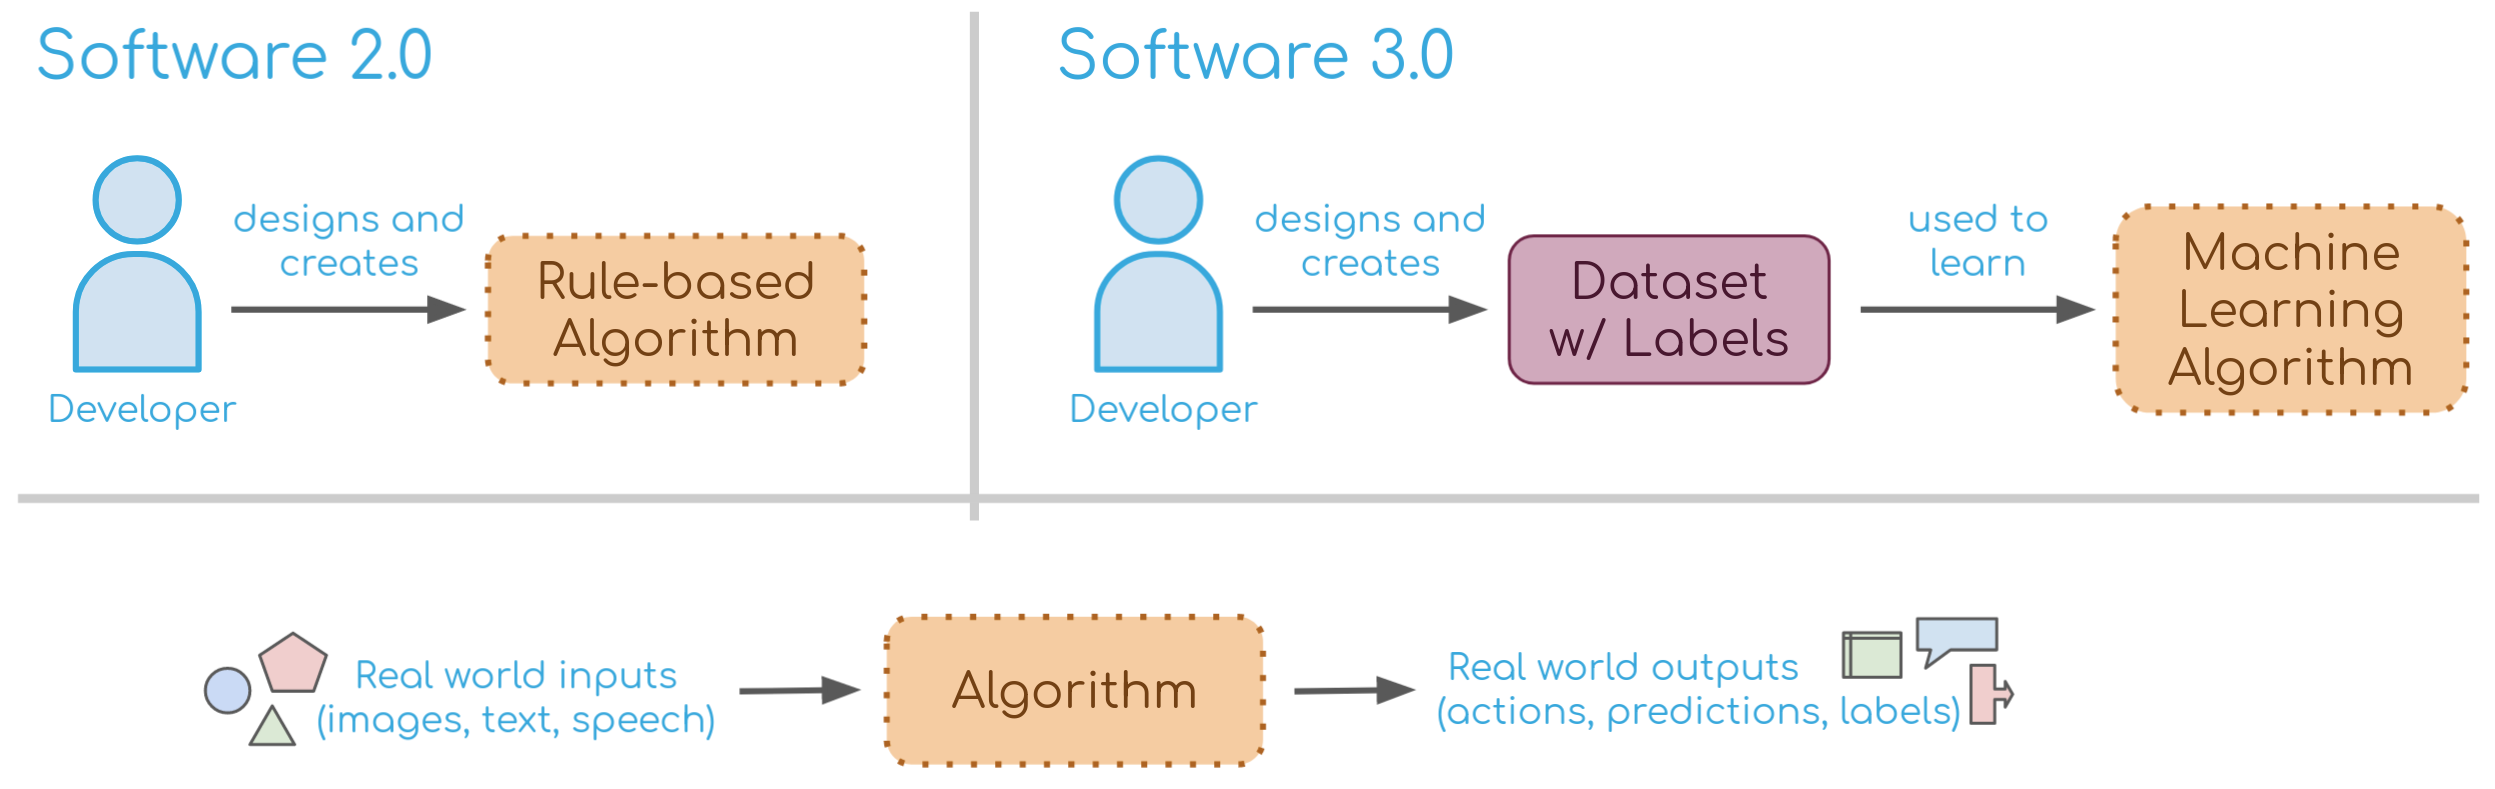
\includegraphics[width=\textwidth]{software3.png}
	\caption{Software 3.0: the developer transitions from writing explicit algorithms to creating and curating datasets which are used to train machine learning models.}
	\label{fig:fig2}
\end{figure}

\subsection{Software 3.0}
See Figure \ref{fig:fig2}. Here is how you add footnotes. \footnote{Sample of the first footnote.}
\lipsum[2]

\section{Project Features}
\label{sec:projectfeatures}

\subsection{Blender Addon}
\lipsum[2]

\subsection{Cloud Backend}
\lipsum[2]

\subsection{User Interfaces}
\lipsum[4] See Section \ref{sec:background}.

\section{Design}
\label{sec:design}

\begin{figure}
	\centering
	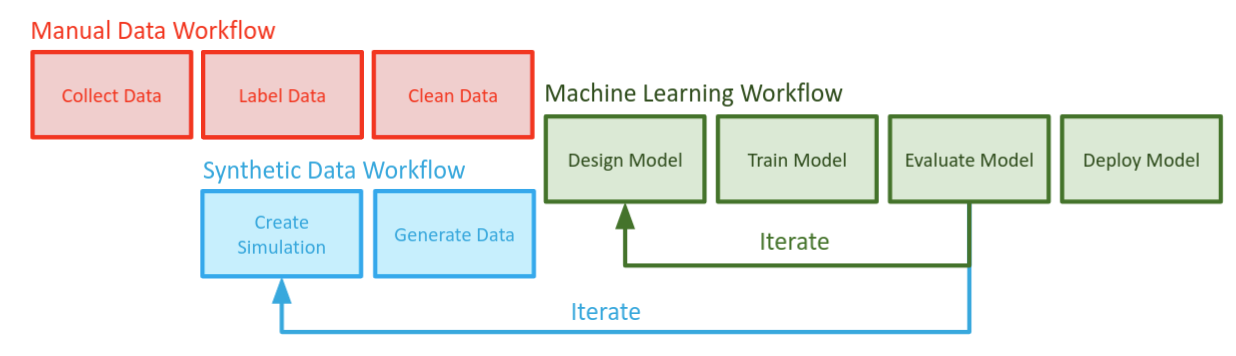
\includegraphics[width=\textwidth]{workflow.png}
	\caption{The Synthetic Data Workflow allows for iteration of the dataset.}
	\label{fig:fig3}
\end{figure}

\section{Workflow}
\label{sec:workflow}
See Figure \ref{fig:fig3}.

\section{Example}
\label{sec:example}

\subsection{Lists}
\begin{itemize}
	\item Domain Randomization of background
	\item Domain Randomization of lighting
	\item Domain Randomization of object
\end{itemize}

See results in the Table~\ref{tab:table}.

\begin{table}
	\caption{Sample table title}
	\centering
	\begin{tabular}{lll}
		\toprule
		\multicolumn{2}{c}{Part}                   \\
		\cmidrule(r){1-2}
		Name     & Description     & Size ($\mu$m) \\
		\midrule
		Dendrite & Input terminal  & $\sim$100     \\
		Axon     & Output terminal & $\sim$10      \\
		Soma     & Cell body       & up to $10^6$  \\
		\bottomrule
	\end{tabular}
	\label{tab:table}
\end{table}

\section{Conclusion}
\label{sec:conclusion}
\lipsum[2]

\bibliographystyle{abbrvnat}
\bibliography{references}

\end{document}
